\section{Results}
In the following section per convention $\lambda$ is the wavelength $d$ is the with of the slit and $z$ is the distance from the screen.\\
As can be seen in figure \ref{fig:single slit interference with 0.04mm width} the theory for a single slit fits the data well however there are
secondary effects easily observable in the tails of the data that per our understanding are partially caused by the nonlinearity of the
photomultiplier and photoelectric sensor, such effects were not taken into account when formulating our theory
However the adjustment can be easily accomplished.
\begin{figure}[H]
    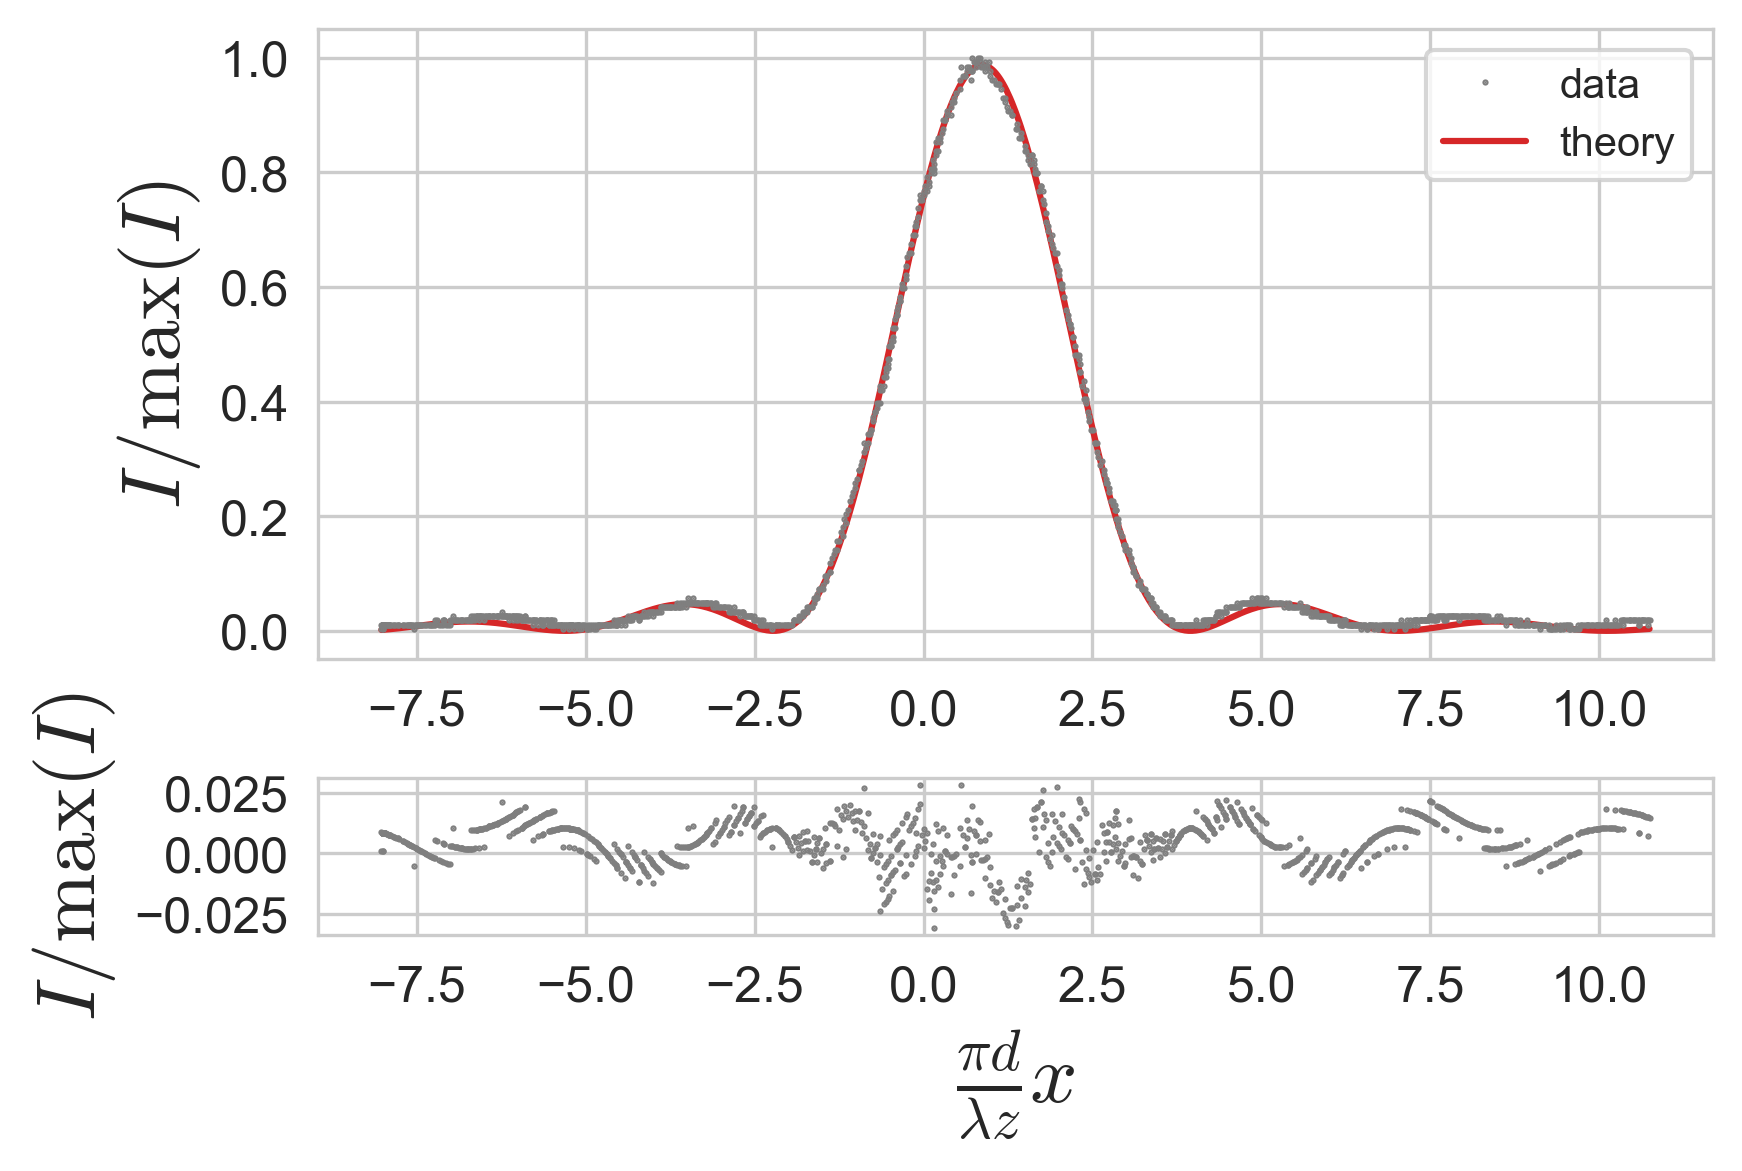
\includegraphics[width=0.9\columnwidth]{figures/single slit interference with 0.04mm width.png}
    \caption{$\lambda$ is the laser wave length $d$ is the width of the slit and $z$ is the distance from the screen}
    \label{fig:single slit interference with 0.04mm width}
\end{figure}
\begin{figure}[H]
	\centering
	\begin{subfigure}{0.5\columnwidth}
		\centering
		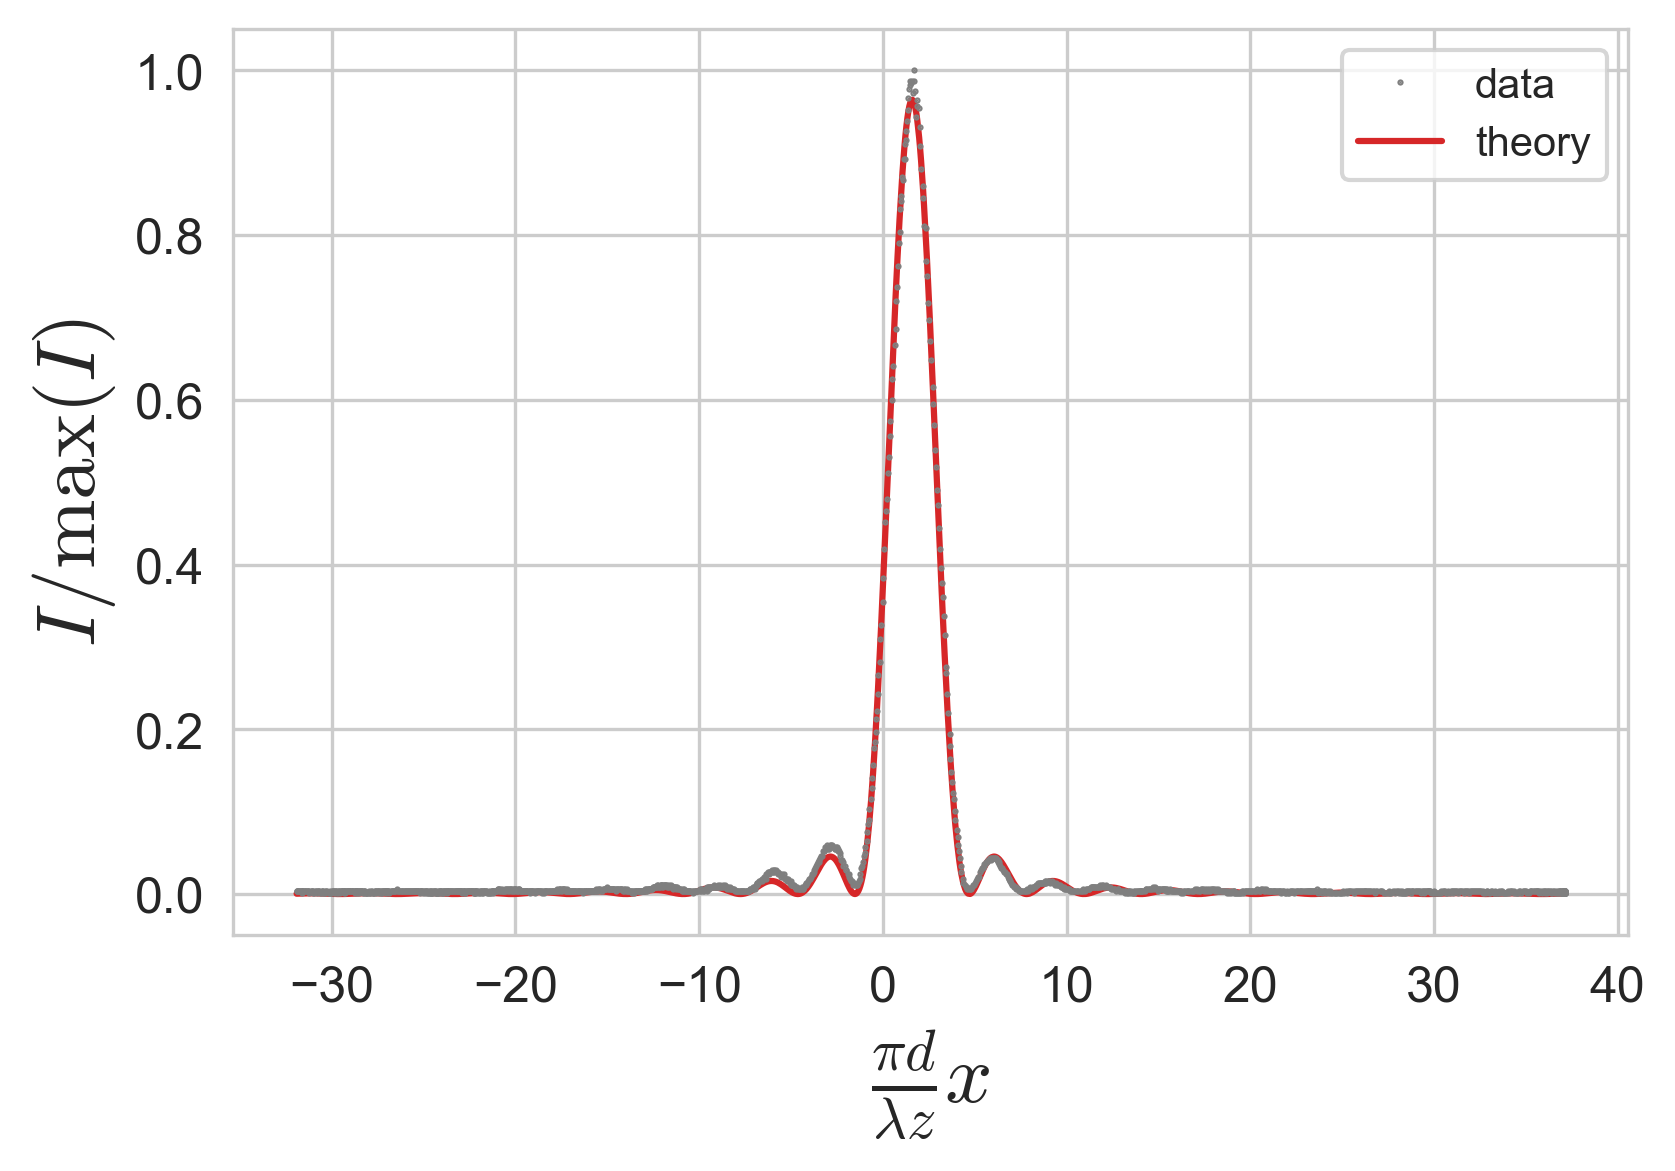
\includegraphics[width=\columnwidth]{figures/single slit interference 0.08mm.png} % first figure itself
		\caption{first figure}
        \label{fig:single slit interference 0.08mm}
	\end{subfigure}\hfill
    \begin{subfigure}{0.5\columnwidth}
        \centering
        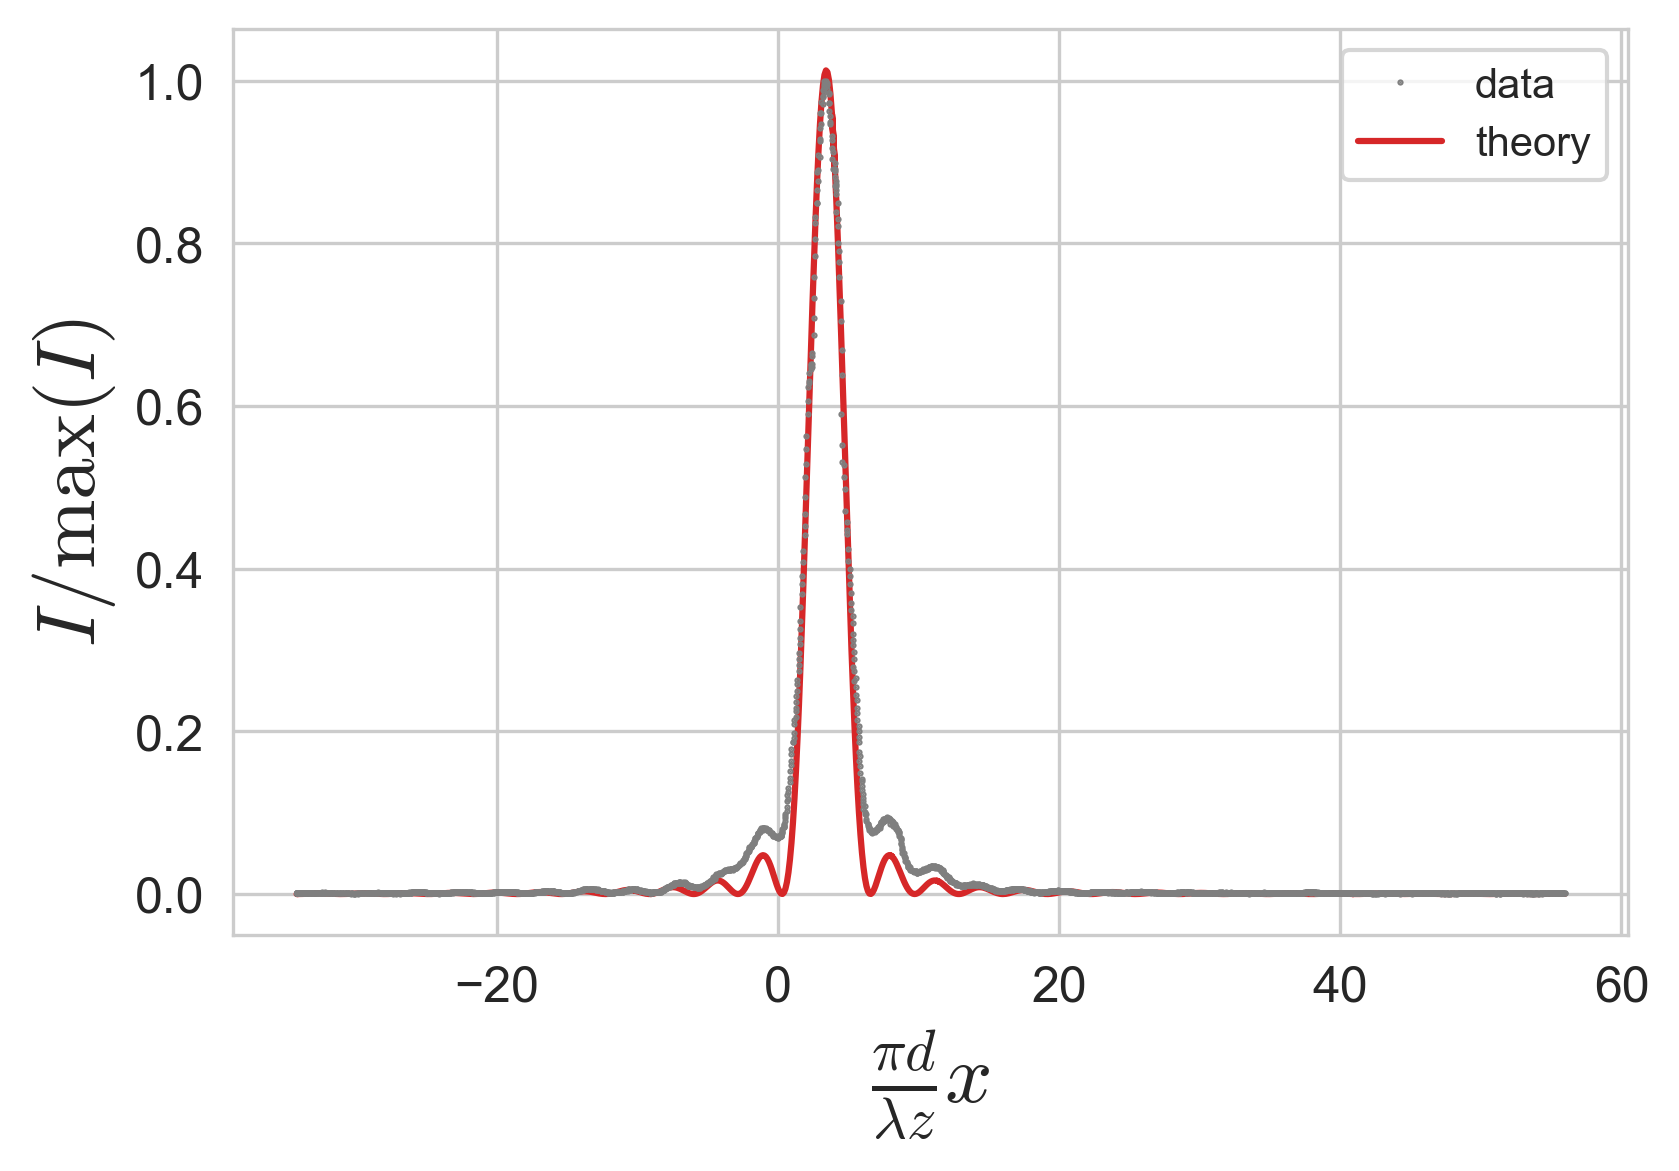
\includegraphics[width=\columnwidth]{figures/single slit interference 0.16mm.png} % second figure itself
        \caption{second figure}
        \label{fig:single slit interference 0.16mm}
    \end{subfigure}
    \label{fig:single slit examples}
\end{figure}

in the case of the periodic diffraction grating "10 lines per mm" the secondary effects are more pronounced especially
the photoelectric sensor's "memory" (The photoelectric sensor has a relaxation period in which to voltage diminishes
therefore after exposure instead of an immediate cut off a slope can be seen as the voltage is recorded with the relation
to the angle which continues to change during said period giving us higher peaks and wider slopes near those peaks)
\begin{figure}[H]
    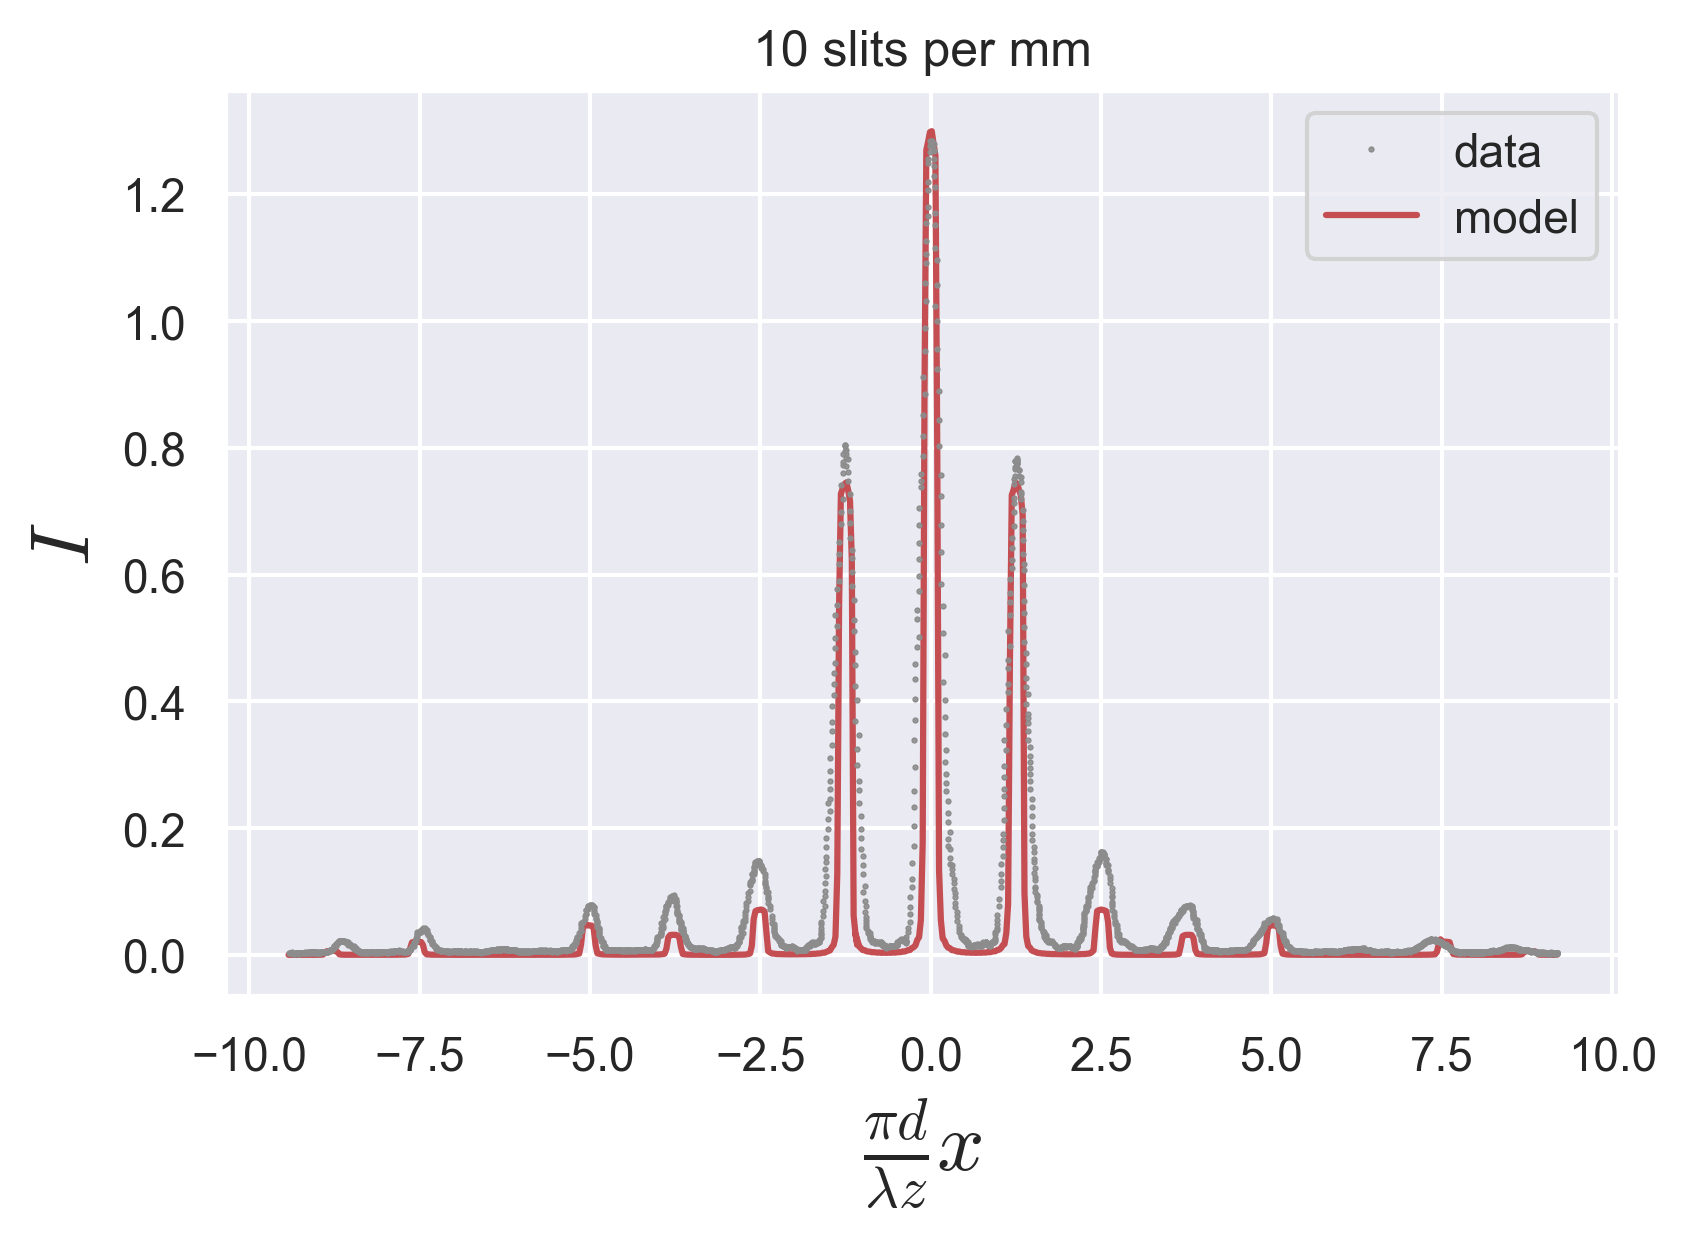
\includegraphics[width=0.9\columnwidth]{figures/10 slits per mm.png}
    \caption{}
    \label{fig:10 slits per mm}
\end{figure}